% !TeX spellcheck = en_US
\documentclass{article}
\usepackage{amsmath}
\usepackage[utf8]{inputenc}
\usepackage{graphicx}
\usepackage{dcolumn}
\usepackage{bm}
\usepackage{showkeys}
\usepackage{ragged2e}
\usepackage{cite}
\newif{\ifmover}
\newif{\ifquitar}
\usepackage{authblk}
\renewcommand{\Affilfont}{\small}
\usepackage{xcolor}
\newcommand{\notaL}[1]{{\color{orange}L: #1}}
\newcommand{\notaVA}[1]{{\color{orange}VA: #1}}
\newcommand{\notaV}[1]{{\bf \em \color{green}VCG: #1}}
\definecolor{Addtext}{RGB}{0,0,255}
\begin{document}

%\title{Thickness optimization in wide range quasi omnidirectional multilayer
% structures}
\title{Optimization of wide-band quasi-omnidirectional 1-D photonic structures}
\author[1,2,3]{Victor Castillo-Gallardo\thanks{email: {\tt
			victor1\_1@hotmail.com}}}
\author[1,2,3]{Luis Eduardo Puente-D\'{i}az}
\author[4]{D. Ariza-Flores}
\author[3]{Hector P\'{e}rez-Aguilar}
\author[2]{W. Luis Moch\'{a}n\thanks{email: {\tt
			mochan@fis.unam.mx}}}
\author[1]{Vivechana Agarwal\thanks{email: {\tt
			vagarwal@uaem.mx}}}
\affil[1]{Centro de Investigaci\'{o}n en Ingenier\'{i}a y
Ciencias Aplicadas, Universidad del Estado de Morelos, Av.
Universidad 1001, Col. Chamilpa, Cuernavaca, Morelos 62209,
M\'{e}xico.}
\affil[2]{Instituto de Ciencias F\'{i}sicas, Universidad
Nacional Aut\'{o}noma de M\'{e}xico, Av. Universidad S/N,
Col. Chamilpa, 62210 Cuernavaca, Morelos, México.}
\affil[3]{Facultad de Ciencias F\'{i}sico Matem\'{a}ticas,
Universidad Michoacana de San Nicol\'{a}s de Hidalgo, Av.
Francisco J. Múgica S/N 58030, Morelia, Mich., M\'{e}xico.}
\affil[4]{CONACyT-Universidad Aut\'{o}noma de San Luis
Potos\'{i}, Karakorum 1470, Lomas 4ta Secc, San Luis Potos\'{i},
S.L.P., 78210, M\'{e}xico.}
%\date{{\small {\today}}}
\maketitle


\begin{abstract}
Porous silicon (PS) is a very versatile material for developing optical
devices based on multilayered structures, since high and low porosity layers
can be synthesized by a simple electrochemical technique. In the present work, the 
average reflectance $<$R$>$ of PS-based mirrors is maximized within a wide 
wavelength and angular range, for different porosity contrasts. Optimization is 
performed to maximize the reflectance for minimum  thickness of the structure in the 
visible (Vis) and near infrarred (NIR) regions of the electromagnetic spectrum.   The 
mirrors are designed using \textit{chirped}-type structures and \textit{stacking} 
sub-mirrors. The chirped structures are found to be more suitable for the Vis range, 
while stacked sub-mirrors are found to be better for the NIR region. Design, fabrication 
and testing of some optimized omnidirectional structures with less than 100 periods has 
been demonstrated.
\end{abstract}

\section{Introduction}

Photonic crystal (PC)-based structures have been extensively investigated due
to their light controlling properties \cite{Joannopoulos2008,Goyal2018}.
Photons entering a PC interact with its periodically varying dielectric constant and
are consequently organized into photonic bands. Analogous to electrons in a
crystal, their propagation is forbidden if their energy lies
within certain regions known as photonic band gaps (PBG's). Thus, the
PC behaves as a mirror if illuminated by light with frequencies
within in a PBG. For several applications it is useful to fabricate
{\em ommnidirectional} mirrors with a wide band gap.  The use of metallic
mirrors is limited due to their relatively large absorption at
visible and near infrared frequencies.  An attractive alternative
consists of low-absorption dielectric
structures,  which may be designed for specific frequency
ranges. One-dimensional (1D) and two-dimensional (2D) PCs have
applications in optoelectronics, optical telecommunications and computing,
laser technology \cite{Lopez2003,Masaya2010}, and radiative cooling applications
\cite{Kumar2020}. The simplest 1D-PC is composed of a finite number
of periodically alternating
layers of high $n_{H}$ and low $n_{L}$ refractive indices, with
corresponding thicknesses $d_H$ and $d_L$ chosen so that their optical
thicknesses are quarter-wavelength
$n_{H}d_{H}=n_{L}d_{L}=\lambda_{0}/4$ at a nominal
wavelength $\lambda_{0}$. This yields a {\em Bragg mirror} (BM)
which might have a large PBG including an omnidirectional gap if the contrast $n_H/n_L$
and the number of periods are large enough. Mirrors with high
reflectance within a wider frequency range may be engineered by
using different nominal wavelengths for different layers.
One way to obtain such structures is to gradually change the width of
the layers as a function of their depth, producing
\textit{chirped}-type structures \cite{Zipock1997}.
Another alternative is to stack BMs, in such a way that their reflection bands partially
overlap each other at the edge, resulting in a wider high-reflection band \cite{Xifre2009}.

On the other hand, different fabrication techniques have been used to obtain omnidirectional (OD) mirrors that operate on the visible and/or near infrared (Vis-NIR) range of the electromagnetic spectrum. For example, Chen et al. \cite{Chen1999},
\notaL{Hay que checar que la puntuación vaya después de las citas,
	para este estilo de citas entre corchetes} reported the fabrication of a 
6-pair TiO$_{2}$/SiO$_{2}$ structure with
an OD band of about 70 nm in the NIR range, employing sol-gel deposition 
method. Park et al. \cite{Park2003}, used molecular beam epitaxy to 
grow a stack of four pairs of GaAs/AlAs layers, followed by its conversion to
GaAs/Al$_{2}$O$_{3}$ layers by selective oxidation of the AlAs 
layers, to obtain an OD with a band from 710 to 950 nm. 
On the other hand, DeCorby et al. \cite{DeCorby2005}, fabricated mirrors by
coupling multiple layers of Ge$_{33}$As$_{12}$Se$_{55}$ chalcogenide glass and
polyamide-imide polymer, deposited by thermal evaporation and spin-casting
respectively, to obtain a 150 nm wide omnidirectional band centered at
1750 nm. Furthermore, Jena et al. \cite{Jena2019},
used sequential asymmetric bipolar pulsed DC magnetron sputtering (for TiO$%
_{2}$ layers) and radio frequency magnetron sputtering (for SiO$_{2}$
layers) to generate TiO$_{2}$/SiO$_{2}$ 1D-PC's and achieved an OD band from
592 to 668 nm. However, these techniques are expensive and they
require sophisticated equipment and long fabrication times. Using PS
is an attractive alternative, since it can be easily manufactured by 
electrochemical etching of crystalline Si in a hydrofluoric 
acid based electrolyte, to obtain a sponge-like nanostructure composed 
of Si and air. By modulating the supplied current and its application 
time during the electrochemical reaction, it is possible to obtain 
multilayer structures allowing for fabrication OD mirrors \cite{Xifre2015,Pavesi2000}.
Although optical filters \cite{Estevez2009,Ariza2014} are the most common
application of PS PC's, they have also been widely used as chemical
sensors \cite{Giusseppe2011,Agarwal2018}, waveguides \cite{Hussel1997} and
for photoluminescence control \cite{Antunez2014}. Recently, the study of
chirped multilayer structures has
increased due to their possible application as flat focusing mirrors \cite{Wu2021,Kozar2017,Cheng2018}.
\notaL{Lens o mirror, no puede ser ambas? De verdad esto es lo que más lo ha popularizado?} 
PS based dielectric optical filters, quasi-OD and OD mirrors have been extensively studied in different
regions of the electromagnetic spectrum, such as the ultraviolet (UV)
\cite{Jimenez2020}, visible \cite{Ariza2012}, and NIR \cite{Bruyant2003} region. 
However, to obtain the desirable high index of refraction
contrast, layers of high porosity have to be employed, which makes the
resulting structures relatively fragile. In addition, use of high porosity makes the fabrication of large structures, with a
very large number of layers, unfeasible. For this reason, in this work
we study different strategies to produce multilayered mirrors
with high reflectance omnidirectional band 
with relatively small thickness and refractive index contrast. 
\notaV{Se omite la frase "Specifically, our aim is to maximize the 
	reflectance $R$ averaged over a wide range of wavelengths $\lambda$ 
	and angles of incidence $\theta$", la idea general esta en la oracion anterior} 

This paper is organized as follows. In Sec. \ref{s:theory} \notaL{No uses números,
	usa referencias a etiquetas para numerar y referir todo} we develop the
methods used to design and calculate the reflectance spectra of the PS
multilayered structures such as chirped structures and mirror
stacks. In Sec. \ref{s:exp} we provide details about the
fabrication of these structures. In Sec. \ref{s:res} we present the numerical
and experimental results corresponding to our proposed structures and compare
them to previous reports. We obtained significantly large band-widths
with relatively thinner structures than reported before. \notaL{Dejo para resultados y
	conclusiones los detalles de con quién comparamos y qué salió.}
Finally, we discuss our conclusions in Section \ref{s:conc}.

\section{Numerical simulation} \label{s:theory}

\notaV{Nombre de la sección propuesta por Dr. David}
\notaL{Pon etiquetas a todo para poderlo referir}
\notaV{Parrafos reescritos por Dr. David}

In this paper, two techniques are developed to design 
multilayer photonic structures. In the first, the wavelength 
($\lambda _{j}$), at which the $j$-th period of the structure 
is designed, is modulated by an increasing function. This can 
be as simple or complex as you like. The proposed function was used to
optimize $<$R$>$ with the Minuit module of PDL (Perl Data Language) \cite{minuit}. 
The other technique for proposing highly reflective structures 
over a wide region of the electromagnetic spectrum is to stack
sub-mirrors tuned to different wavelengths. For each 
sub-mirror the dispersion relation is analyzed.

For the analysis of the propagation of electromagnetic fields 
through multilayer systems, we employ the transfer matrix 
method based on Puente-Díaz et al. formalism \cite{Puente2020}. 
In spite some equivalent formulations have been proposed to 
obtain the optical properties of multilayer systems 
\cite{Mochan1987,Ortiz2020,Chavez2020}, here we use a 
recently developed formalism for the numerically stable 
calculation of the reflectance of large multilayer systems. 
Briefly describing, 
we assume a 1D system with variations along the $z$ direction 
and consider an incident linearly polarized beam of light 
(either TE or TM polarization) that propagates throughout 
the structure. The reflectance and transmittance are given by 
$R=|r|^{2}$ and  $T=\beta \left\vert t\right\vert ^{2}$,
respectively, with \cite{Puente2020}
\begin{equation}
	r=\mp \frac{Z_{0}M_{11}+M_{12}-Z_{0}Z_{s}M_{21}-Z_s
		M_{22}}{Z_{0}M_{11}-M_{12}-Z_{0}Z_{s}M_{21}+Z_{s}M_{22}},  \label{rBloch}
\end{equation}%
and
\begin{equation}
	t=\frac{2Z_{\zeta
	}}{Z_{0}M_{11}-M_{12}-Z_{0}Z_{s}M_{21}+Z_{s}M_{22}},  \label{tBloch}
\end{equation}%
where $Z_0$ and $Z_s$ are the impedances of the vacuum 
and the substrate, respectively. $\beta =\text{Re}Z_{0}/\text{Re}Z_{s}$ is chosen for 
TE polarization while $\beta=\text{Re}Z_{s}/ 
\text{Re}Z_{0}$ for TM polarization. The upper sign 
$-$ in Eq. (\ref{rBloch}) and the subscript 
$\zeta =s$ in Eq. (\ref{tBloch}) are chosen for 
the case of TE polarization, while the lower sign 
$+$ and the subscript $\zeta =0$ correspond to TM 
polarization. Moreover, sub-index $0$ and $s$ 
refer to the incident and substrate media, respectively.
Furthermore, $M_{ij}$ are the elements
of the transfer matrix which relates
the electromagnetic fields of all interfaces in the structure through


\begin{equation}
\resizebox{\textwidth}{!}{$\displaystyle{
	M=\frac{1}{Z^{+}-Z^{-}} \left( 
	\begin{array}{cc}
		Z^{+}\text{exp}\left( iKD\right) -Z^{-}\text{exp}\left( -iKD\right)  & 
		-2iZ^{+}Z^{-}\sin KD \\ 
		2i\sin KD & Z^{+}\text{exp}\left( -iKD\right) -Z^{-}\text{exp}\left(
		iKD\right) 
	\end{array}%
	\right) \text{.}}$}  
\label{MsBloch}
\end{equation}
%}
In this case, $Z^{\pm }$ can be obtained as 
\begin{equation}
	Z^{\pm }=-\frac{\widetilde{M}_{12}}{\widetilde{M}_{11}-\Lambda _{\pm }}\text{,}  \label{ZBloch}
\end{equation}%
being 
\begin{equation}
	\Lambda _{-}=\frac{1}{2}\text{tr}\widetilde{M}\pm i\sqrt{1-\left( \text{tr}\widetilde{M}/2\right)
		^{2}}\text{,}  \label{LBloch}
\end{equation}%
where the sign that satisfies the relation $\left\vert \Lambda
_{-}\right\vert >1$, and $\Lambda _{+}=\Lambda _{-}^{-1}$ is chosen.
Moreover, tr corresponds to the trace and $\widetilde{M}_{ij}$ $\left( i,j=1,2\right) 
$ denote the elements of the usual transfer matrix $\widetilde{M}$ of the $N$-layer
system, that is, 
\begin{equation}
	\widetilde{M} = \prod \limits_{j=1}^{N}%
	\begin{bmatrix}
		\cos k_{j}d_{j} & iZ_{j}\sin k_{j}d_{j} \\ 
		iY_{j}\sin k_{j}d_{j} & \cos k_{j}d_{j}%
	\end{bmatrix}%
	,  \label{Mcoef}
\end{equation}%
where 
\begin{equation}
	k_{j}=\sqrt{\epsilon _{j}q^{2}-Q^{2}}  \label{kj}
\end{equation}%
is the normal component (to the interfaces) of the wave vector, $Z_{j}$ is
the corresponding surface impedance, $Y_{j}=1/Z_{j}$ is the surface
admittance, $\epsilon _{j}=n_{j}^{2}$ is the permitivity (for simplicity we
assumed all media were nonmagnetic, with permeability $\mu _{i}=1$), $%
q=\omega /c=2\pi /\lambda $ is the free-space wavenumber corresponding to
the wavelength $\lambda $ and 
\begin{equation}
	Q=n_{0}q\sin \theta _{i}  \label{Snell}
\end{equation}%
is the projection of wavevector onto the interfaces, 
which is conserved according to Snell's law, with 
$\theta _{i}$ the angle of incidence. The surface 
impedances are given by $Z_{j}=q/k_{j}$ for TE 
polarization and $Z_{j}=k_{j}/q\epsilon _{j}$ for 
TM polarization. The complex refractive index of the porous layers were 
obtained through the Bruggeman's effective medium 
theory, which has been reported to adequately reproduce 
the PS optical parameters \cite{Giusseppe2011,Pap2006,Estrada2018}.


\section{Experimental details}\label{s:exp}


Some of the proposed photonic structures were synthesized through anodic
etching of a (100) oriented, $p$-type Boron doped, crystalline Si wafer with
resistivity 0.002-0.005 $\Omega \cdot $cm, under galvanostatic conditions
\cite{Canham1990,Escorcia2007}. The electrochemical anodization process was
performed at room temperature, with an electrolyte of aqueous
hydrofluoric acid (HF) (48$\%$ of
wt) and ethanol (99.9$\%$ of wt) in 1:1 volumetric proportion, respectively.
However, as it is not desirable to use very high
porosity contrasts due to structure fragility and electrolyte
diffusivity problems \cite{Ariza2011}, the current
densities were chosen as 35 and 305 $\text{mA}/\text{cm}^{2}$, 
with corresponding porosities of 51\% and 76\%, respectively.
The porosity of the layers was obtained by a previous calibration
curve through a gravimetric technique \cite{Pap2006}. The 
etching rate of PS was obtained by synthetizing single layers under 
similar conditions and measuring their thicknesses through Scanning 
Electron Microscopy (SEM). Absolute reflectivity measurements were 
carried out with a Perkin Elmer Lambda 950 UV/Visible 
spectrophotometer with a variable angle universal reflectance 
accessory (URA) for different incident angles $\theta _{i}=10^{\circ 
}$, $20^{\circ }$, $30^{\circ }$, $40^{\circ }$, $50^{\circ }$ and 
$60^{\circ }$ using non-polarized light. The maximum and minimum 
values of $\theta _{i}$ were constrained by the angular range of the 
equipment accessory URA.


\section{Results and discussion}\label{s:res}


In this section we present optimized calculations of the reflectance
of different multilayered omnidirectional wide-band mirrors and we
compare the results with experimental spectra taken from
the corresponding samples at several angles of
incidence. Sec. \ref{ss:chirped} is devoted to chirped-type Bragg
mirrors while Sec. \ref{ss:stacked} is devoted to structures made of
stacked sub-mirrors.


\subsection{Chirped-type Bragg mirrors}\label{ss:chirped}


Here we study multilayered structures where the thicknesses for each
pair $j=0\ldots N_p$ of layers are tuned to a wavelength $\lambda_j$ which changes
gradually with the depth of the layer, according to
\begin{equation}
\lambda_{j}=\lambda_{\min }+\left(\lambda_{\max }-\lambda_{\min}\right) f\left(\frac{j-1}{N_p-1}\right),\label{Dis}
\end{equation}%
where $\lambda_{\min }$ and $\lambda_{\max }$ are the minimum and
maximum {\em design} wavelengths respectively, $N_p$ is the number of periods in the structure and $f(\xi)$ is some smooth function that 
goes from 0 to 1 as its argument goes from surface ($\xi=0$) to the 
substrate ($\xi=1)$. We only consider increasing functions $f$ due to 
the high absorption of PS in the ultraviolet region which decreases in 
the visible and becomes negligible in the near infrared, so, the first 
periods are syntonized in the UV-Vis regions. We consider the 
following classes of functions:
\begin{equation}
f_{1}\left(\xi \right) =\xi^{\alpha },  \label{F1}
\end{equation}
\begin{equation}
f_{2}\left(\xi \right) =\frac{1}{2}\left(\xi^{\alpha }+\xi^{\beta}\right)
\label{F2}
\end{equation}
and%
\begin{equation}
f_{3}\left(\xi\right) =Ax^{\alpha }\left(1-\xi\right) +\xi^{\beta },  \label{F3}
\end{equation}
where $\alpha$, $\beta$ and $A$ are parameters to optimize \notaV
{Agregue} in order to maximize the average reflectance. The function
$f_{1}$ (Eq. (\ref {F1})) represents simple increasing profiles,
restricting  $\alpha>0$. The function $f_2$ is an arithmetic averages
of two functions of the type $f_{1}$ with different
powers $\alpha$ and $\beta$ \notaL{A ¿no debe ser 1/2 a fuerza, para
que $f_2(1)=1$? \notaV{Si}}. The function $f_{3}$ (Eq. (\ref{F3})) is 
designed so that the first addend dominates near the surface and the 
second addend prevails near the substrate, to allow different behaviors 
at the edges \notaV{Omitted "at UV and IR end"} of the spectrum. 
\notaV{Se replanteo el resto del parrafo} The parameters 
that were optimized to obtain the maximum average reflectance were 
$\alpha$, $\beta$, $A$ and $N_{p}$. The reflectance $R(\lambda, 
\theta)$ of the resulting structures was calculated in two regions of 
the electromagnetic spectrum. The first region was chosen from 350 to 
1400 nm and second one was selected from 400 to 3000 nm, both in the 
angular range of $0^\circ$ to $90^\circ$. Additionally, in the first 
region the minimum design wavelength was optimized and the maximum 
design wavelength was set at 1400 nm, while in the second region the 
wavelengths were set at 850 and 3000 nm, respectively. The 
calculations were carried out using the Perl Data Language (PDL) and 
its interface with the MINUIT \cite{minuit} minimization package. The 
optimized parameters corresponding to a porosity contrast of 51 and 76\% 
are shown in Table \ref{tab:tableA}. 

\notaV {En caso de ser necesario "In the supplementary information we include the parameters for the porosity tests of $30/76 \% $ and $42/76 \%$."}

\notaV{Se replanteo el contenido} 

\begin{table}[!ht]
	\begin{center}
		\label{tab:tableA}
\caption{Optimized parameters yielding the highest average reflectance $<$R$>$  for the profile classes $f_1$, $f_2$ and $f_3$ (Eqs. (\ref{F1}) - (\ref{F3}))}
		\resizebox{\textwidth}{!}{ 
		\begin{tabular}{|c|c|c|c|c|c|c|c|c|}
			\hline % <-- Toprule here
			\textbf{Func-}&\multicolumn{3}{|c|}{\textbf{Parameters}} &\textbf{Periods}&\textbf{Thick-}&\textbf{OD}&\textbf{$\lambda_{0}$}&\textbf{$R_{Ave}$}\\
		\textbf{tion}&$\alpha$&$\beta$&A&$N_{p}$&\textbf{ness} ($\mu$m)& \textbf{width} ($\mu$m)&($\mu$m)&$\%$\\
			\hline
			$f_{1}$&0.24&---&---&222&86.1&0.30&1.150&89\\
			$f_{2}$&0.37&1.06&---&102&35.9&0.22&1.110&88\\
			\textcolor{red}{$f_{3}$}&\textcolor{red}{1.23}&\textcolor{red}{0.54}&\textcolor{red}{0.18}&\textcolor{red}{63}&\textcolor{red}{21.6}&\textcolor{red}{0.25}&\textcolor{red}{1.125}&\textcolor{red}{89}\\
			\hline
			\textcolor{red}{$f_{1}$}&\textcolor{red}{1.20}&\textcolor{red}{---} &\textcolor{red}{---} & \textcolor{red}{90}&\textcolor{red}{60.4}&\textcolor{red}{2.15}&\textcolor{red}{1.925}&\textcolor{red}{92}\\
			$f_{2}$&1.08&1.86&--- &105&61.7&2.00&2.000&89\\
			$f_{3}$&1.01&1.95&0.20&102&62.3&2.05&1.975&90\\
			\hline
		\end{tabular}
	}
	\end{center}
\end{table}

\notaL{No es claro en el texto cómo se obtiene $N_p$. Se mencionaba
  una minimización del ancho, pero no recuerdo cómo se minimizó a la
  vez que se maximizaba la reflectancia. ¿Fue minuit? ¿Fue a ojo?}
\notaV{$N_{p}$ lo proporciona minuit para cada una de las funciones propuestas y del m\'{i}nimo lo tom\'{e} para hacer el experimento}

According to table \ref{tab:tableA}, in the first region, the function 
$f_{3}$ modulates the best distribution of the periods in the smallest 
thickness and the proposed photonic structure has the highest 
reflectance. Furthermore, this structure has an OD gap with a reflectance 
$R>0.90$ of 250 nm centered at 1125 nm, as shown in Fig. \ref{Fig1}(b). This 
structure will be synthesized and we will call it S-1. In the second region, the 
proposed structures have very similar thicknesses and reflectance 
spectra; however, the one with the smallest thickness and the maximum 
reflectance is the one designed from the function $f_{1}$. This 
structure will also be synthesized and we will call it S-2. The 
calculated reflectance spectra of S-2 are shown in Fig. \ref{Fig1}(d). 
This structure has a very wide region where $ R(\lambda, \theta)> 
0.90$, which is located from 850 to 3000 nm and in an angular range 
of $0^\circ$ to $70^\circ$. So, we can say that S-2 has a 
quasi-OD (q-OD) gap of 2150 nm centered at 1925 nm. On the other hand, 
the profiles of the functions (with the optimized parameters) that 
modulate the distribution of the $j-th$ period tuned to the $\lambda_ 
{j}$, in the first analysis region, are shown in Fig. \ref{Fig1}(a). 
In Fig. \ref{Fig1}(c), the profiles of the functions related to the 
second region are plotted. In these figures, it is observed that the 
profiles are very similar in each region of analysis. For example, in 
the first analysis region, it is necessary that the photonic 
structures have the least number of periods tuned in the areas where 
the SP is absorbing and that they are the first periods of the 
structure. In the second region, it is only necessary that the periods 
have an adequate ordering.
\begin{figure}[!ht]
		\label{Fig1}
	\begin{center}
		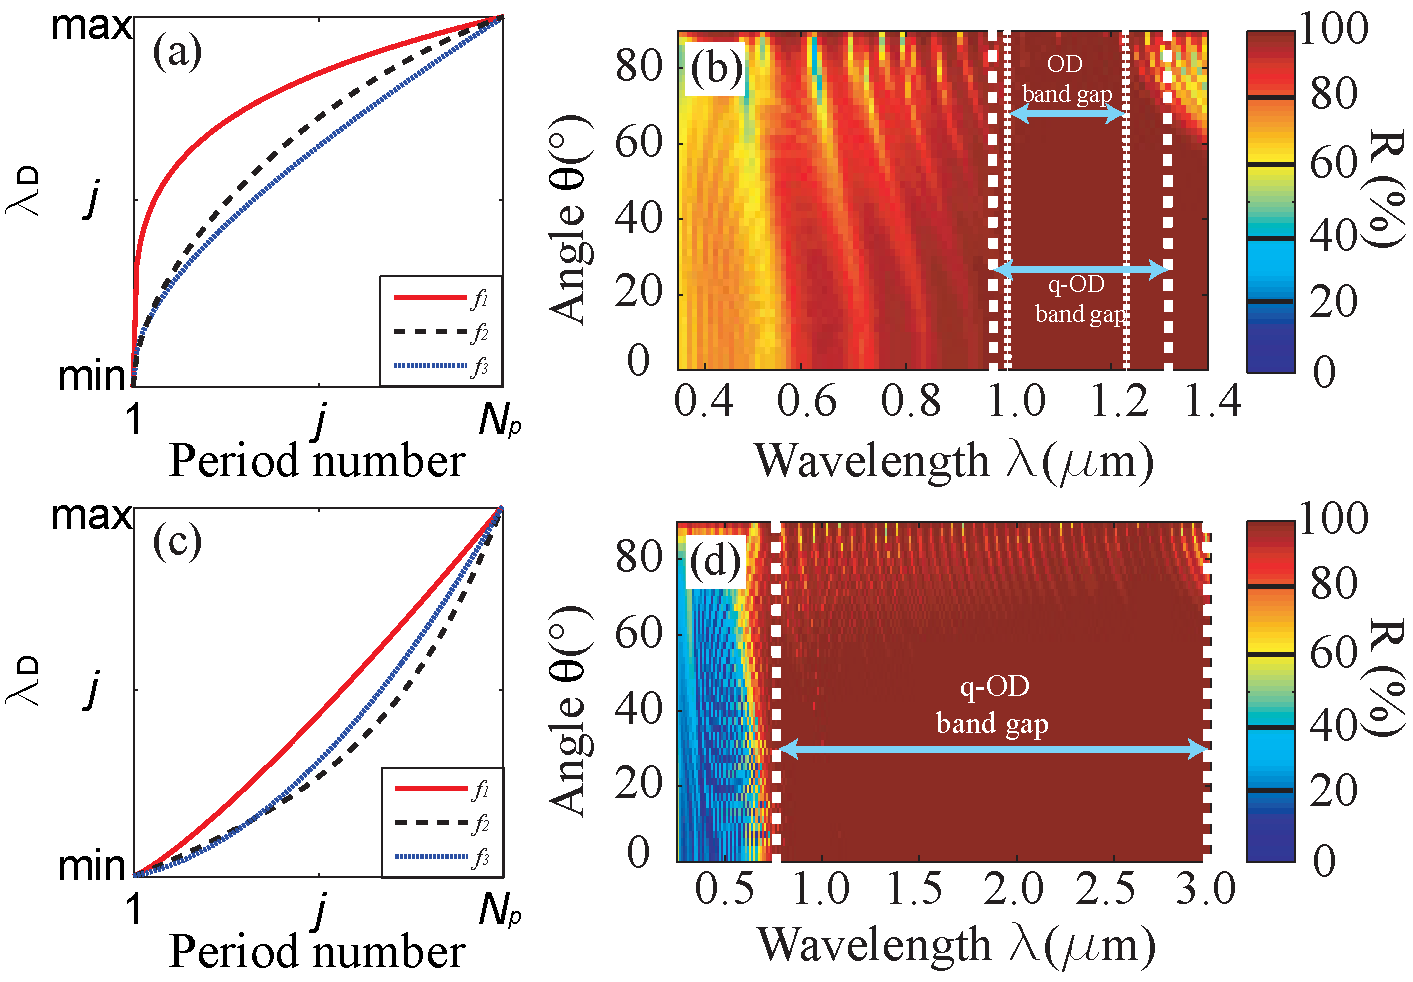
\includegraphics[width=\textwidth]{F1Alternativa.pdf}
	\end{center}
	\caption{Profiles of the optimized functions that modulate the distribution of the $j-th$ period tuned to the design $\lambda_ {j}$ for the analyzed structures in the region (a) from 350 to 1400 nm and (c) from 400 to 3000 nm. Reflectance spectra of the optimized structures in the region (b) from 350 to 1400 nm and (d) from 400 to 3000 nm. The dotted lines delimit the area where R $> 90\%$ and the dashed lines indicate the quasi-OD region. In the first region there is an OD gap and in the second region there is a quasi OD gap. Calculations are for non-polarized light.}
\end{figure}


We fabricate the optimized structures (S-1 and S-2) and measure their 
reflectance spectra at various angles of incidence $\theta$. Due to 
experimental limitations, we restrict our results to the case of 
unpolarized light. In Fig. \ref{Fig2}(a), the calculated and measured 
reflectance are compared from 350 to 1400 nm for different angles of 
incidence ($\theta=10^\circ$, $20^\circ$, $30^\circ$, $40^\circ$, 
$50^\circ$, and $60^\circ$) for S-1. They have very similar 
characteristics. For example, for $\lambda>700$ nm and 
$10^\circ < \theta < 40^\circ$, the spectrum differs by less than $5\%$ and for 
$\theta > 40^\circ$ both spectra are qualitatively consistent but the 
measured reflectance is less than the calculated one. This difference 
can be attributed, in part, to the scattering of light at real 
interfaces, which generally have a certain roughness 
\cite{Theiss1994,Chavez2020,Ortiz2020} that we have not taken into 
account in our theory. Reflectance was measured using unpolarized 
light. Due to the limitations of the spectrophotometer, it is not 
possible to perform measurements for $\theta>60^\circ$ and thus 
check the OD gap. Therefore, in this angular range, we will limit 
ourselves to saying that the structure has a quasi-omni-directional 
bandgap (R$\left(\lambda,\theta \right)>90\%$) located between 980 and 
1340 nm.
\begin{figure}[!ht]
	\label{Fig2}
	\begin{center}
		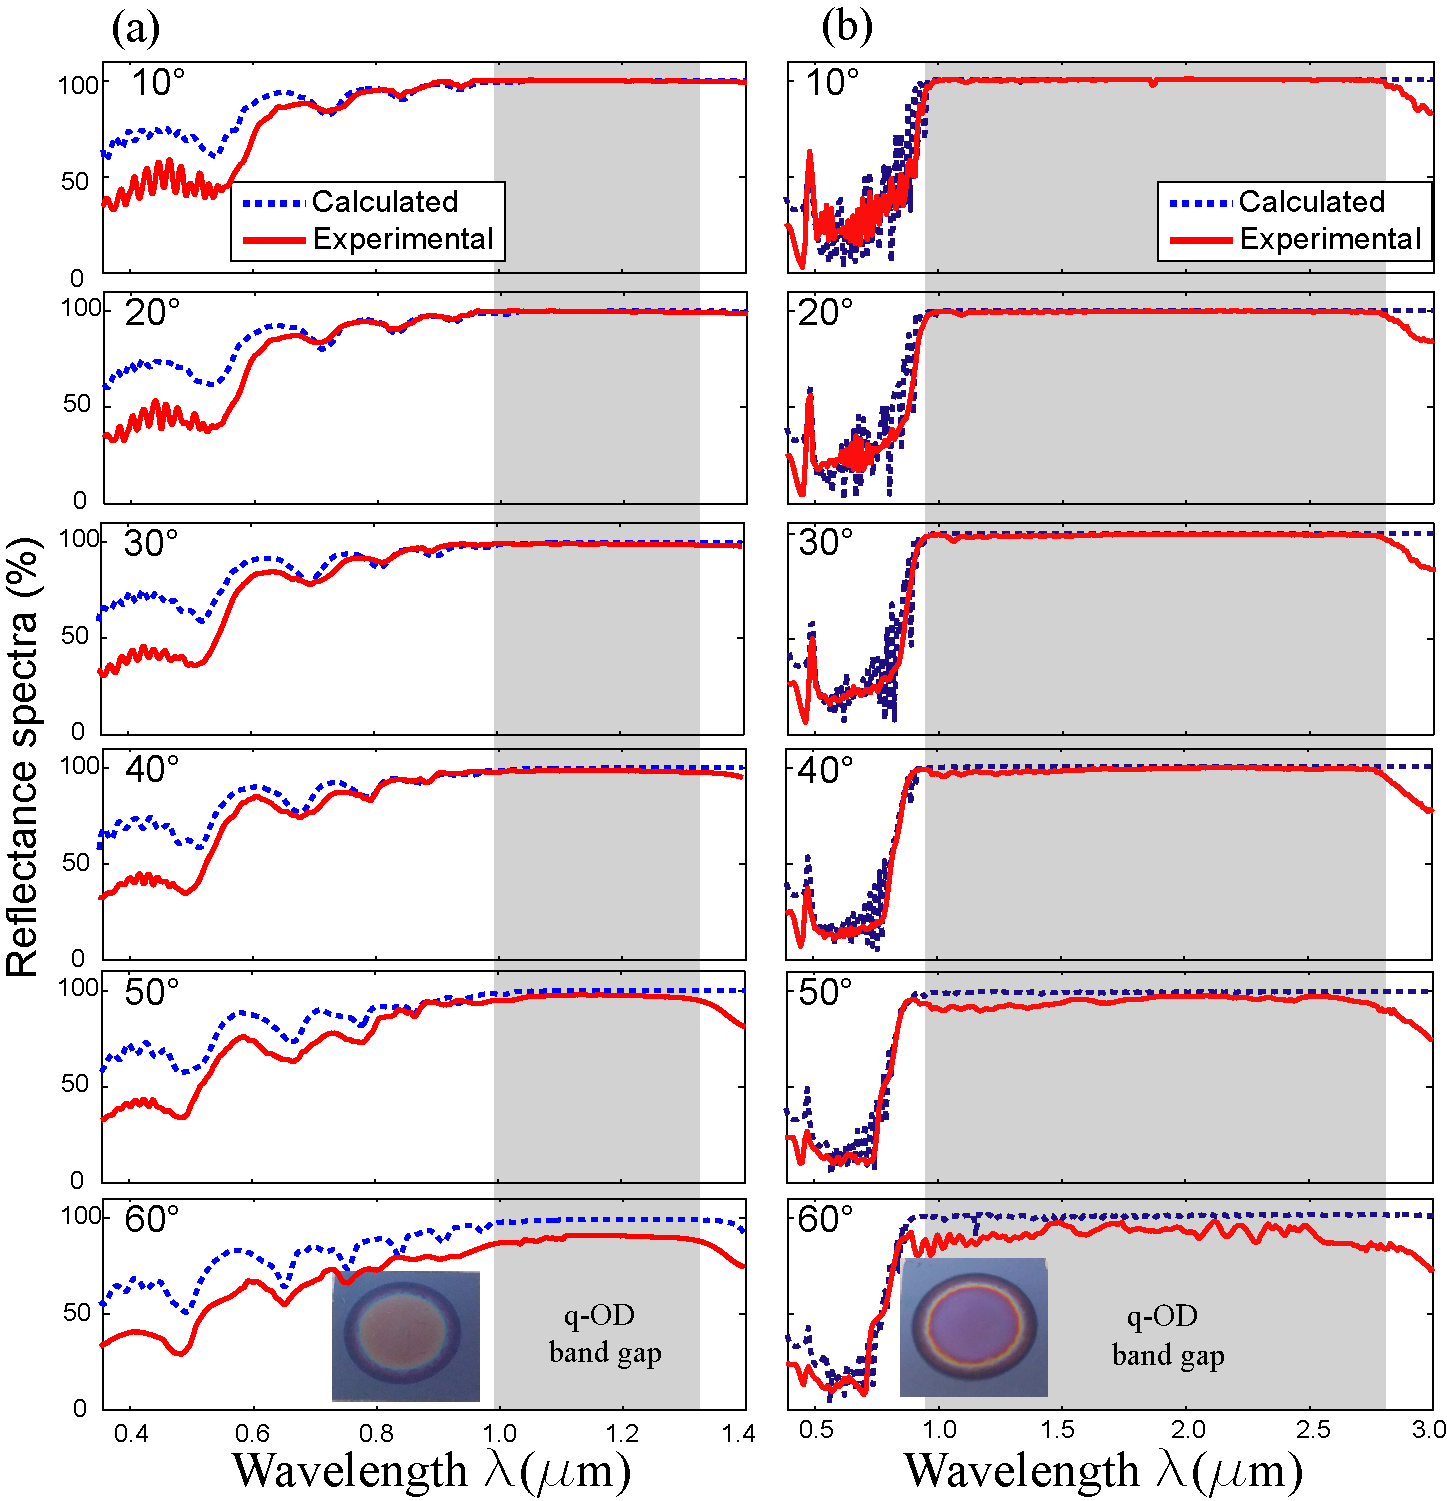
\includegraphics[width=\textwidth]{F2Alternativa.pdf}
	\end{center}
	\caption{Reflectance spectra calculated and measured at different 
	angles of incidence for structure (a) S-1 and (b) S-2. Reflectance spectra are for non-polarized light. The gray band indicates the region where the reflectance is greater than  $90\%$. This region corresponds to the quasi OD gap of the structure. Inset: photograph of the synthesized structure.}
\end{figure}

On the other hand, Fig. \ref{Fig2}(b) shows the comparison of the 
calculated reflectance spectra and the spectra measured in the range 
from 400 to 3000 nm and the aforementioned incidence angles for S-2. 
These spectra are also very similar. The difference between the 
calculated and measured spectra at longer wavelengths, can be 
attributed to an increase of imperfections such as wavy layers and 
more roughness for deeper layers, due to a more restricted diffusivity 
of the electrolyte as the thickness of the structure is increased 
\cite{Negro2003,Vincent1993}. According to the results obtained, this 
structure has a wide quasi-omnidirectional gap ($R>0.90$) of 1800 nm 
centered at 1880 nm.



\subsection{Photonic structure with sub-mirrors stacking}\label{ss:stacked}

Another technique for designing structures that reflect across a wide range of the 
electromagnetic spectrum is to stack sub-mirrors tuned to different wavelengths. For 
example, Agarwal et al. \cite{Agarwal2003} proposed to stack sub-mirrors as follows: 
first select the $\lambda_{1}$ value from the initial sub-mirror, then subsequent 
$\lambda$ values obey a simple relation $\lambda_{i+1} + \lambda_{i}=2+i$, where $i$ 
represents the sub-mirror number. Furthermore, Estrada-Wiese et al. \cite{DelRio2018} 
developed a method that combines three stochastic optimization algorithms together with 
a  narrow space search methodology to obtain a customized and optimized 
PC configuration. 

In this technique, we continue to use the 
propagation of Bloch waves in periodic structures, since this allows 
us to know the frequencies that cannot propagate through the 
structure. These are obtained by analyzing the expression
\begin{equation}
	 \cos (KD) = \frac{1}{2} \text{Tr}M,   \label{Dispersion}
\end{equation}
where $D$ is the thickness of the sub-mirror, $\pm K$ 
represents the Bloch vector that propagates in the sub-mirror 
\cite{Mochan1987, Mochan1988, Perez2018}, Tr denotes the trace 
and $M$ is the matrix given by Eq. \ref{MsBloch}. This equation 
is limited by the minimum and maximum values that the 
cosine function can take. Also, if the value of 
$\left\vert\text {Tr} \left(M \right) \right\vert$ is $>2$, it 
indicates that this frequency will not be able to propagate 
through the structure.

It is common to imagine that the stacking of the sub-mirrors is as 
follows: that the PBG of the $j+1-th$ mirror starts at the edge of the 
PBG of the $j-th$ mirror and stack enough mirrors until covered the 
bandwidth of the desired range. However, with this configuration, the 
reflectance has minimum values at each edge of to contiguous PBG.
On the other hand, the number of periods of each sub-mirror is an 
important parameter due to its direct dependence on the magnitude and 
width of the photonic forbidden band. Since the structures are 
synthesized using porous silicon, it is essential to minimize the 
number of periods corresponding to the sub-mirrors of the visible 
region. For these reasons, the design of the structure was carried 
out in two different ways: in the first, constant periods were 
considered and in the second, a constant number of periods was 
assigned for the interval from 400 to 800 nm (a period for 
$\lambda_{D}<500$ nm, two periods for $500 <\lambda_ {D} < 650$ nm 
and three periods for $650<\lambda_ {D}<800$ nm) and for 
$\lambda_{D}>800$ nm, the number of periods was variable. In both 
designs, the optimal overlap of two consecutive PBGs was obtained that 
maximized reflectance. Reflectance spectra were calculated from 400 to 
3000 nm in the spectral range of $0^\circ$ to $90^\circ$. 
Table \ref{tab:table2} shows the number of periods of each sub-mirror 
($Np_{se}$), the total number of stacked sub mirrors ($N_{se}$), the 
thickness of the structure, the optimal overlap of two consecutive 
PBGs and the average reflectance. The first block corresponds to 
sub-mirrors with a constant number of periods, while the second block 
corresponds to sub-mirrors with a variable number of periods according 
to the design wavelength. 
\begin{table}[htbp]
	\begin{center}
		\caption{Parameters that maximize the reflectance of photonic structures.}
		\label{tab:table2}
		\begin{tabular}{|c|c|c|c|c|}
			\hline % <-- Toprule here
			\textbf{$Np_{se}$}&{\textbf{$Np_{se}$}} &\textbf{Thickness}&\textbf{Overlap}&\textbf{$R_{Ave}$}\\
			&&($\mu$m)& \textbf{PBG $\%$}&$\%$\\
			\hline
			1&98&43.2&95&91.0\\
			3&31&42.5&81&91.8\\
			5&17&41.9&68&92.0\\
			\hline
			4&25&38.7&74&92.3\\			\textcolor{red}{6}&\textcolor{red}{18}&\textcolor{red}{41.5} &\textcolor{red}{78} & \textcolor{red}{95.35}\\
			10&13&45.4&56&95.34\\
			\hline
		\end{tabular}
	\end{center}
\end{table}

According to table \ref{tab:table2}, the structure that has the highest 
reflectance is in the second block. We will call this structure S-3. In 
S-3, the overlap of two consecutive PBGs is $78\%$, their thickness is 
41.5 $\mu$ m, and the average reflectance is $95.3\%$. Additionally, 
S-3 is made up of 18 sub-mirrors tuned to the following wavelengths 
400, 460, 510, 570, 640, 720,810,910, 1020, 1150, 1290, 1450, 1630, 
1830, 2060, 2320, 2610, and 2860 nm. The calculated and measured 
reflectance spectra of S-3 are shown in Fig. \ref{Fig3}.
\begin{figure}[!ht]
\begin{center}
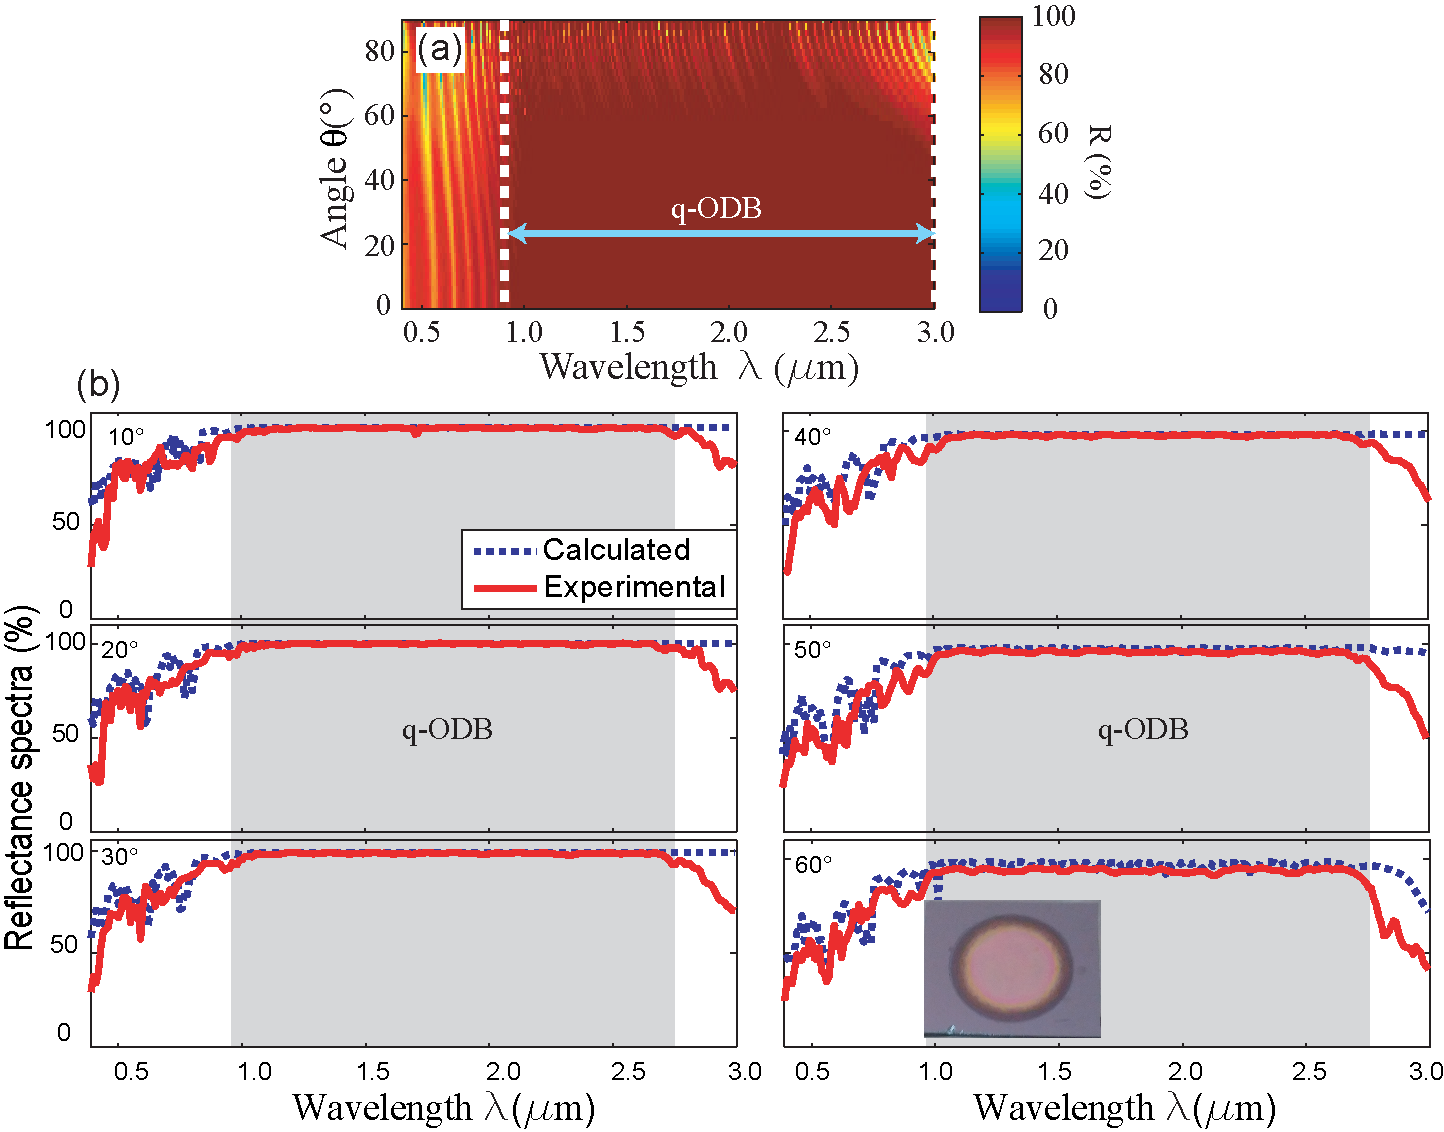
\includegraphics[width=\textwidth]
{F3Alternativa.pdf}
\end{center}
\caption{ (a) Calculated reflectance for the optimized structure S-3. (b) Comparison 
	between the measured and calculated reflectance spectra at several angles of 
	incidence. Reflectance spectra are for non-polarized light. The gray band indicates 
	the region in which the reflectance is greater than 90$\%$.  Inset shows a 
	photograph with a top view of the synthesized structure.}
\label{Fig3}
\end{figure}

The reflectance mapping shown in Fig. \ref{Fig3}(a) reveals a quasi omnidirectional 
mirror in the range from 950 to 2900 nm, and angular range between $0^\circ$ and 
$60^\circ$. It is also observed that at incidence angles $>$70${{}^\circ}$, for long 
wavelengths the reflectance decreases and has oscillations, which are attributed to the 
greater penetration of the electromagnetic field within the structure, as shown by 
Puente-D\'{\i}az, et al. \cite{Puente2020}. In Fig. \ref{Fig3}(b) we compare the 
calculated and measured reflectance for the structure S-3, at several angles of 
incidence. Although, the quasi omnidirectional wavelength range of the synthesized 
structure is slightly smaller than the calculated one, from 950 to 2750 nm, the measured 
PBG is almost twice as wide as a recently reported PS chirped structure \cite{Chavez2020}.

Finally, table \ref{tab:table3} shows some porous silicon based OD mirrors designed to operate in the NIR 
region and the width of the omnidirectional band gap is compared with the structures 
analyzed in the present study. The table reveals that the porous silicon based 
structures ST-B and ST-C have the widest gap width, being 1.36 times greater than the 
largest reported work until now in the NIR region \cite{Wu2021}.

\begin{table}[!ht]
	\begin{center}
		\caption{Summary of the development in porous silicon based ODBMs designed in the NIR region.}
		\label{tab:table3}
		\begin{tabular}{|c|c|c|c|}
			\hline % <-- Toprule here
		\textbf{Reference}&\textbf{Year}&\textbf{ODBM range}&\textbf{ODBM width}\\
			 & &(nm)&(nm)\\%&\textbf{ST-B}&\textbf{ST-C}\\
			\hline % <-- Midrule here
Bruyant, et al. \cite{Bruyant2003} & 2003 & 1100-1440 & 340 \\
Xifre-P\'{e}rez, et al. \cite{Xifre2005} & 2004 & 1297-1615 & 318\\
Estevez, et al. \cite{Estevez2009} & 2009 & 950-1456 & 506 \\
Chavez, et al. \cite{Chavez2020} & 2020 & 1000-2000 & 1000 \\
Wu, et al. \cite{Wu2021} &2021&1284-2605&1321 \\
			\hline % <-- Bottomrule here
			\begin{tabular}{c|c}
					&ST-A\\
					This article&ST-B\\
				&ST-C\\
			\end{tabular}&
			\begin{tabular}{c}
			\\
			\\
			\\
			\end{tabular}&
		\begin{tabular}{c}
			980-1340\\
			980-2780\\
			950-2750\\
		\end{tabular}&
		\begin{tabular}{c}
			360\\
			1800\\
			1800\\
		\end{tabular}\\
		\hline % <-- Bottomrule here
	\end{tabular}
	\end{center}
\end{table}


\section{Conclusion}\label{s:conc}
\notaV {Se replantean las conclusiones}.

We have designed, fabricated and characterized highly 
reflective q-OD (angular range of $0-60^\circ$) 
multilayer structures, with a wide spectral range, 
optimized through two techniques: chirping and stacking 
Bragg-type sub-structures. Numerical calculations were 
carried out by employing the transfer matrix method, 
incorporating a Perl Minuit module in order to maximize 
the average reflectance of the structures. Some of the 
optimized structures were manufactured with PS dielectric 
multilayers and compared with their simulations. For the 
chirping method, a couple of structures were fabricated, 
one with thicknesses of 21.6 $\mu$m and other with thickness 
of 60.4 $\mu$m, resulting in reflectivity q-OD bands of 
360 nm and 1800 nm, centered at 1160 nm and 1925 nm, 
respectively. For staking sub-structures method we 
obtained a 41.5 $\mu$m thickness mirror with a q-OD 
band of 1800 nm centered at 1850 nm. Therefore, the second technique is found to be better as it results in structures with relatively
less thickness  along with noticeable improvement 
in average reflectance. Additionally, the analysis 
techniques developed here can be used to optimize 
reflectance with other refractive index contrasts 
in PS multilayers or in different systems with other 
types of materials. Such proposed structures could 
be used as mirrors for solar concentrators, flat 
focusing reflectors, thermal regulators, or, if 
defects are included, as filters or remote 
chemical/biosensors with a wide angular independent response.


\section*{Acknowledgments}
This work was partially supported by Consejo Nacional de Ciencia y
Tecnolog\'{i}a through grant No. 256243, C\'{a}tedras
Conacyt program 1577, and by DGAPA-PAPIIT UNAM under grant IN111119. 
HPA also express his gratitude to the Coordinaci\'{o}n 
de la Investigaci\'{o}n Cient\'{i}fica de la Universidad 
Michoacana de San Nicol\'{a}s de Hidalgo. 
%\end{acknowledgments}


\bibliographystyle{unsrt}
\bibliography{Bibliografia}
\end{document}
